\begin{figure}[h]
    \centering
    \caption{Proyección del SGP como porcentaje del PIB}
    \label{fig:sgp_forecast}
    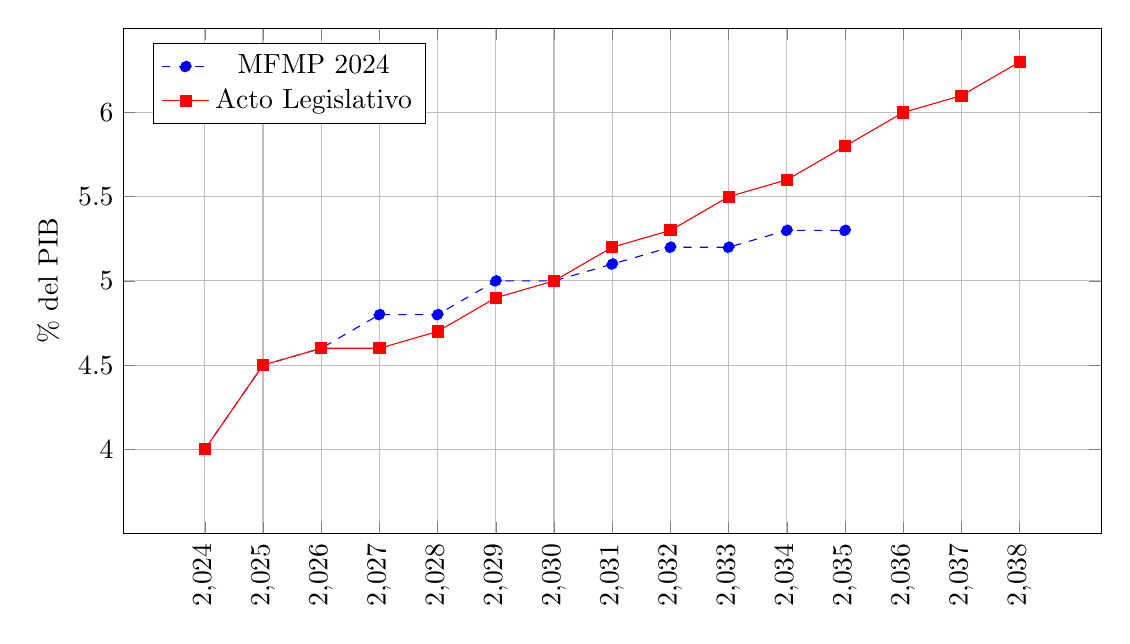
\begin{tikzpicture}
        \begin{axis}[
            width=14cm, height=8cm,
            ylabel={\% del PIB},
            xtick={%2023,
            2024,2025,2026,2027,2028,2029,2030,2031,2032,2033,2034,2035,2036,2037,2038},
            xticklabel style={rotate=90, anchor=east},
            ymin=3.5, ymax=6.5,
            legend pos=north west,
            grid=major,
            ytick={4,4.5,5,5.5,6},
        ]

        % MFMP 2024
        \addplot[color=blue, mark=*, dashed] coordinates {
            %(2023,3.4) 
            (2024,4.0) (2025,4.5) (2026,4.6) (2027,4.8)
            (2028,4.8) (2029,5.0) (2030,5.0) (2031,5.1) (2032,5.2)
            (2033,5.2) (2034,5.3) (2035,5.3)
        };
        \addlegendentry{MFMP 2024}

        % Acto Legislativo
        \addplot[color=red, mark=square*] coordinates {
            %(2023,3.4) 
            (2024,4.0) (2025,4.5) (2026,4.6) (2027,4.6)
            (2028,4.7) (2029,4.9) (2030,5.0) (2031,5.2) (2032,5.3)
            (2033,5.5) (2034,5.6) (2035,5.8) (2036,6.0) (2037,6.1) (2038,6.3)
        };
        \addlegendentry{Acto Legislativo}

        \end{axis}
    \end{tikzpicture}
    \vspace{0.1cm}
    \par\footnotesize{\textit{Fuente: Elaboración propia y MFMP 2024 del Ministerio de Hacienda.}}
\end{figure}
